O rețea socială este o platformă online folosită de oameni pentru a construi relații sociale cu alte persoane care au același interese,
activități, sau legături din viața reală. Rețelele de socializare asigură utilizatorilor modalități de a posta idei, fotografii, videoclipuri și postări, 
pentru a informa persoane din comunitatea lor despre activități online sau din viața reală. Depinzând de tipul de platformă, membrii au posibilitatea de 
a contacta alte persoane. Varietatea serviciilor deja disponibile în mediul online provoacă o dificultate în a defini ce este o rețea de socializare,
și totuși sunt câteva caracteristici comune\cite{SocialNetworks}.
\begin{itemize}
    \item Aplicațiile de tip rețea de socializare necesită conexiune la internet.
    \item Conținutul generat de utilizator este esențial în rețelele de socializare.
    \item Utilizatorii pot crea conturi ce sunt proiectate și întreținute de organizația ce deține rețeaua de socializare.
    \item Serviciile oferite de o rețea de socializare oferă utilizatorilor posibilitatea de conectare cu alți oameni sau grupuri de persoane.
\end{itemize}

\section{Concepte}
     \subsection{Single Page Aplication - SPA}
    Aplicațiile de tipul SPA sunt aplicații web ce încarcă o singură pagină HTML\footnote{HTML - „HyperText Markup Language” este un limbaj 
de marcare utilizat pentru crearea paginilor web ce pot fi afișate într-un navigatoar web.} și actualizează dinamic pagina în timp ce 
utilizatorul interacționează cu aplicația. SPA-urile utilizează AJAX\footnote{AJAX - „Asynchronous JavaScript and XML” este o tehnică 
de programare pentru crearea de aplicații web interactive. Intenția este să facă paginile web să devină mai rapide și deci mai acceptate, 
prin schimbul în fundal al unor cantități mici de date cu serverul, astfel încât să nu fie nevoie ca pagina să fie reîncărcată la 
fiecare acțiune a utilizatorului. Aceasta are ca scop creșterea interactivității, vitezei și ușurinței în utilizare a aplicațiilor web.} și HTML5 pentru a crea aplicații web responsive, fară a reîncărca pagina.
Totodată asta înseamnă ca se întâmplă mai multe pe partea de client, în JavaScript. Într-o aplicație de tipul SPA, după ce este încarcată
prima pagină, toate interacțiunile se întâmplă prin intermediul apelurilor AJAX (Fig.~\ref{fig:spa}). Aceste apeluri AJAX  returnează informații în format JSON\footnote{
JSON - „JavaScript Object Notation” este un format de reprezentare și interschimb de date între aplicații.}.
\begin{figure}[h]
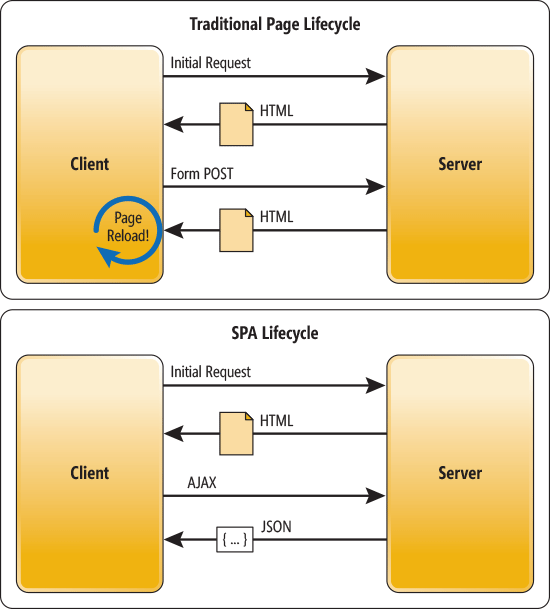
\includegraphics[height=0.8\linewidth]{spa.png}
\centering
\caption{Comparație aplicație web obișnuită cu SPA.\cite{SPA}}
\label{fig:spa}
\end{figure} 
    \subsection{RESTful Web Services}
Representational state transfer(REST) sau RESTful web services reprezintă o cale de oferi interoperabilitate între calculatoare pe internet.
Serviciile REST permit accesarea și manipularea resurselor web folosind un set uniform și predefinit de operații fără stare. Există și 
alte tipuri de servicii web, cum ar fi SOAP\footnote{SOAP - „Simple Object Access Protocol„ este un protocol pentru schimbul de informație structurată
într-o implementare de servicii web.}, ce expun propriul set de operații.

    Resursele web au fost definite pentru prima dată ca și documente sau fisiere identificate de propriul URL\footnote{URL - 
„Uniform Resource Locator” este o secvență de caractere standardizată, folosită pentru denumirea, localizarea și identificarea unor resurse de pe Internet, inclusiv 
 documente text, imagini, clipuri video, expuneri de diapozitive, etc.}. Într-un serviciu REST
cererile către un URI vor primi un răspuns definit într-un limbaj de structurare a datelor cum ar fi XML\footnote{XML - „Extensible Markup Language„ 
este un limbaj de marcare ce definește un set de reguli.} sau JSON. Răspunsul va confirma dacă a fost făcută o modificare asupra resursei accesate,
și poate returna o legătură către o altă resursă relevantă. Folosind protocolul HTTP\footnote{HTTP - „Hypertext Transfer Protocol” este un protocol la nivel de aplicație pentru 
distribuție, sisteme de colaborare, informare hypermedia.}
operațiile sunt predefinite de verbele HTTP(GET, POST, PUT, DELETE, OPTIONS, PATCH,etc).
    Deoarece serviciile REST folosesc un protocol fără stare și operații standard, acestea tind a fi performante, fiabile și extensibile. 
\begin{figure}[h]
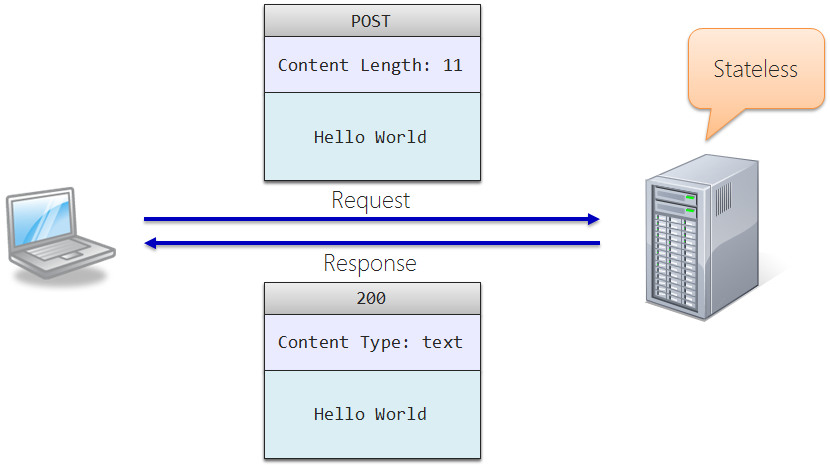
\includegraphics[height=0.4\linewidth]{rest.png}
\centering
\caption{Exemplu cerere-răspuns.}
\label{fig:rest}
\end{figure} 
\section{Tehnologii}
     \subsection{PostgreSQL}
PostgreSQL este un sistem de baze de date relaționale. Este disponibil gratuit sub o licență open-source de tip BSD\footnote{
Licențele BSD sunt o familie de licențe pentru software liber folosite mai ales de sistemele de operare BSD. BSD este prescurtarea de la expresia 
engleză \textit{Berkeley Software Distribution}, o distribuție a sistemului de operare Linux.}. PostgreSQL nu este controlat de nici o companie,
 își bazează dezvoltarea pe o comunitate răspândită la nivel global, precum și câteva companii 
dezvoltatoare. PostgreSQL rulează proceduri stocate în diverse limbaje de programare, cum ar fi Java, Perl, Python,
Ruby, C/C++ și propriul PL/pgSQL ce este similar cu Oracle PL/SQL. Conține sute de funcții proprii iar procedurile stocate 
pot fi scrise în C și încărcate în baza de date ca și librării, adăugându-se astfel flexibilitate în extinderea funcționalităților.
    \subsection{Java}
Java este un limbaj de programare orientat-obiect, proiectat de către James Gosling la \textit{Sun Microsystems} (acum filială 
Oracle) în anul 1990, lansat ulterior în 1995. Limbajul împrumută o mare parte din sintaxă de la C și C++, dar are un model al 
obiectelor mai simplu și prezintă mai puține facilități de nivel jos. Un program Java compilat, corect scris, poate fi rulat fără 
modificări pe orice platformă care e instalată o mașină virtuală Java. Acest nivel de portabilitate este posibil deoarece sursele Java 
sunt compilate într-un format standard numit bytecode (Fig.~\ref{fig:java-compiler}) care este intermediar între codul mașină (dependent de tipul calculatorului) și 
codul sursă (Fig.~\ref{fig:JVM}). Mașina virtuală Java este mediul în care se execută programele Java.
\begin{figure}[h]
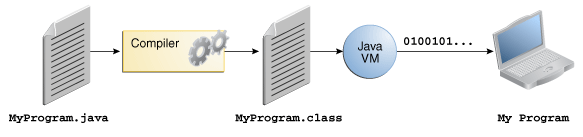
\includegraphics[height=0.2\linewidth]{java-compiler.png}
\centering
\caption{Procesul de dezvoltare au unui program Java.}
\label{fig:java-compiler}
\end{figure} 
\begin{figure}[h]
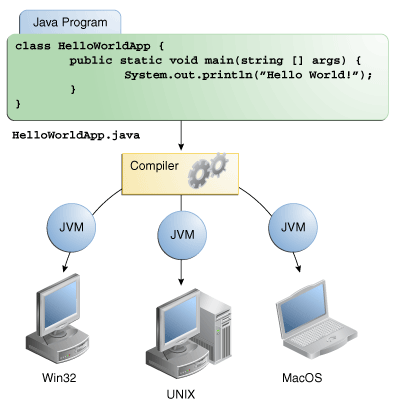
\includegraphics[height=0.6\linewidth]{JVM.png}
\centering
\caption{Aplicați Java capabilă sa ruleze pe mai multe tipuri de platformă.}
\label{fig:JVM}
\end{figure} 
    \subsection{Spring}
Spring este un soft-cadrul\footnote{Soft-cadru - este o platformă universală, un software reutilizabil pentru a dezvolta aplicații.} 
open-source, oferit de \textit{Pivotal Team}, pentru limbajul de programare Java. Prima versiune a fost scrisă de Rod Jhonson, ce a lansat soft-cadrul în octombrie 2002.
A fost lansat prima dată sub licență Apache 2.0 în iunie 2003. Ultima versiune stabilă Spring 4 a fost lansată pe 10 iunie 2016.

Componenta centrală a soft-cadrului este containerul IoC\footnote{IoC - este un acronim de la „Inversion of control” și reprezintă un 
șablon de programare ce este folosit pentru a creste modularitatea și extensibilitatea unei soluții software.}, ce oferă o flexibilitate 
în configurarea și managementul obiectelor Java reflection. Containerul este responsabil pentru crearea, apelarea și managementul 
instantelor de obiecte. Obiectele create de către container sunt numite și \textit{Beans}. Containerul poate fi configurat încărcând fișiere
XML sau detectând adnotările Java 
de pe clasele de configurări. Obiectele pot fi obținute prin injectarea dependințelor. Injectarea dependințelor este un șablon de programare 
în care containerul pasează instanțele obiectelor după nume, altor obiecte prin constructor sau proprietăți(Fig.~\ref{fig:spring-ioc}).
\begin{figure}[h]
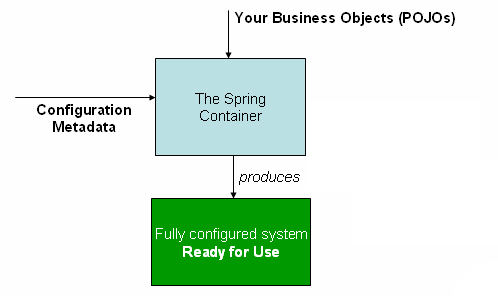
\includegraphics[height=0.5\linewidth]{spring-ioc.png}
\centering
\caption{Containerul Spring IoC.}
\label{fig:spring-ioc}
\end{figure} 

    \subsubsection{Spring Boot}
Spring Boot este un soft-cadru proiectat special pentru a ușura crearea și configurarea aplicațiilor Spring. Acesta oferă adnotări pentru
configurarea rapidă au unui nou proiect Spring. Spring Boot nu este implementat de la zero, ci este o extensie a soft-cadrului Spring(Fig.~\ref{fig:spring-boot}), ce 
ușurează scrierea testelor unitare, scurtează durata de dezvoltare și crește productivitatea\cite{SpringBoot}.
\begin{figure}[h]
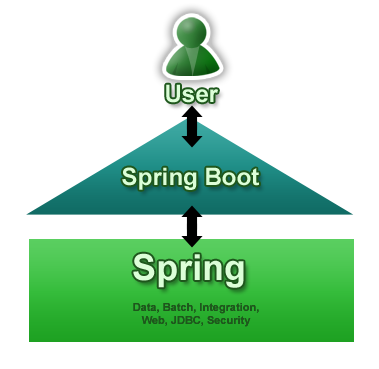
\includegraphics[height=0.4\linewidth]{spring-boot.png}
\centering
\caption{Spring Boot extensie a soft-cadrului Spring.}
\label{fig:spring-boot}
\end{figure} 

    \subsubsection{Spring Data JPA}
Spring Data JPA este oferă un template JPA pentru integrarea cu aplicațiile Spring. JPA(Java Persistent API) este o specificație pentru 
persistența obiectelor într-o aplicație și este folosit pentru a reduce din complexitatea obiectelor de tip entitate(entity beans).

    \subsubsection{Spring Security - OAuth2}
Spring Security OAuth oferă suport pentru folosirea Spring Security cu standardul OAuth2.

    OAuth2 este un protocol standard de autorizare, ce înlocuiește protocolul original OAuth creat în 2006. OAuth2 este concentrat pe 
simplitatea oferită clientului în autorizarea de aplicații web, desktop sau mobile\cite{OAuth2}.
    \subsection{Hibernate}
Hibernate este un ORM(Object relational mapper) ce a fost conceput de către Gavin King ca o alternativă la soluția oferită de EJB2. Scopul original a fost de 
a oferi capabilități mai bune decât cele oferite de EJB2, reducând complexitatea și furnizând noi funcționalități.

Hibernate este un soft-cadru open-source folosit pentru maparea unui obiect orientat
obiect la o bază de date relațională. Caracteristica primară este maparea claselor java la tabelele bazei de date și maparea tipurilor de date Java
la tipurile de date SQL. Hibernate oferă posibilitatea de a folosi configurări, in fișiere XML sau adnotări, pentru mentenanța schemei bazei de date.
Totodată oferă și posibilități de construi relații \textit{1-N}, \textit{N-N}, \textit{1-1} între clase.
    
    \subsection{MapStruct}
MapStruct este un generator de cod open-source ce simplifică major implementarea mapărilor dintre clase diferite, bazându-se pe convenții și configurări.

Aplicațiile pe mai multe straturi de obicei necesită maparea dintre diferite modele de obiecte(de exemplu
entități și DTO-uri(Data Transfer Objects)).Scrierea codului pentru astfel de mapări poate duce la apariția de erori.
MapStruct are rolul de a simplifica și automatiza pe cât posibil acest proces. În comparație cu alte
soft-cadre de mapare, codul pentru mapări este generat în timpul compilării ceea ce asigură o performanță
înaltă prin informarea rapidă a dezvoltatorului cu privire la erorile apărute.
\cite{MapStruct}.
    \subsection{Maven}
Maven o soluție open-source oferită de \textit{Apache Software Fundation}
 pentru construirea și managementul proiectelor in Java. 
 Funcționalitățile sale principale sunt descrierea procesului de construire a software-ului și descrierea dependențelor 
 acestuia. Un fișier XML descrie proiectul care urmează să fie construit, dependențele acestuia sau ale module și 
 componente de care depinde, ordinea în care se execută construirea, directoarele și plug-in-urile necesare. Maven descarcă 
 dinamic bibliotecile Java și plug-in-uri necesare, din unul sau mai multe repository-uri\cite{Maven}.
    \subsection{TypeScript}
    TypeScript este un limbaj de programare open-source dezvoltat de către \textit{Microsoft}. A fost făcut public in octombrie 2012,
 abia după doi ani de dezvoltare internă la \textit{Microsoft}. Este un superset cu o sintaxă 
strictă de JavaScript ce adaugă tipuri de date opționale și clase. TypeScript devenind astfel un limbaj orientat obiect.
    TypeScript poate fi folosit pentru a construi aplicații JavaScript pentru partea de client sau de server(folosind NodeJs). Fiind 
conceput pentru a folosit în dezvoltarea aplicațiilor complexe acesta compilează codul TypeScript in cod JavaScript. TypeScript oferă suport pentru
clase, module și expresii lambda așa cum este propus în standardul ECMAScript 6\cite{TypeScript}.
    \subsection{Node.js}
Node.js este o  open-source pentru aplicații scalabile de tip server și client. Aplicațiile Node.js dezvoltate limbajul de programare 
JavaScript, și pot fi rulate în runtime-ul Node.js pe Linux,Mac OS X, sau Windows, fără a fi necesare modificări.
Aplicațiile Node.js folosesc un singur fir de execuție deși platforma rulează pe mai multe fire. Node.js folosește 
intern motorul Google V8 JavaScript pentru execuția codului și majoritatea modulelor de bază sunt scrise în JavaScript. 
Node.js are o bibliotecă asincronă pentru operații I/O, socket și comunicații HTTP. Node.Js poate fi un server web datorită
suportului pentru socket și HTTP.
    \subsection{Angular 2}
Angular 2 este o platforma open-source pentru dezvoltarea de aplicații web ce are la bază limbajul de programare TypeScript. Angular 2 este dezvoltat
de \textit{Google} și a fost lansat pe 23 martie 2017, fiind compatibil versiunea anterioară cu Angular 2. Angular 2 a reprezentat o rescriere totală
a soft-cadrului AngularJS. Principale caracteristici ale platformei prezentate în figura de mai jos(Fig.~\ref{fig:angular}) sunt:
\begin{itemize}
    \item Modulele cu rolul de încapsula functionalitățile aplicației.
    \item Componentele reprezentând o unitate compusă din View, Model si Styles.
    \item Template-uri reprezentând un view cu sintaxă specială pentru a îmbina limbajul de marcare HTML cu funcționalitatea de data-binding.
    \item Metadata reprezentând datele ce unesc view-ul cu view-modelul, style-urile,etc.
    \item Data-binding\footnote{Data binding este o tehnică de sincronizare a datelor dintre producător și consumator.} reprezentând sincronizarea datelor dintre view și view-model.
    \item Serviciile ce încapsulează și refolosesc logica ce nu aparține de view, oferind astfel posibilitatea de a fi folosite în mai multe părți alea aplicației.
    \item Injectarea de dependințe necesare în componente, ce oferă extensibilitate și testabilitate platformei.
\end{itemize}
\begin{figure}[h]
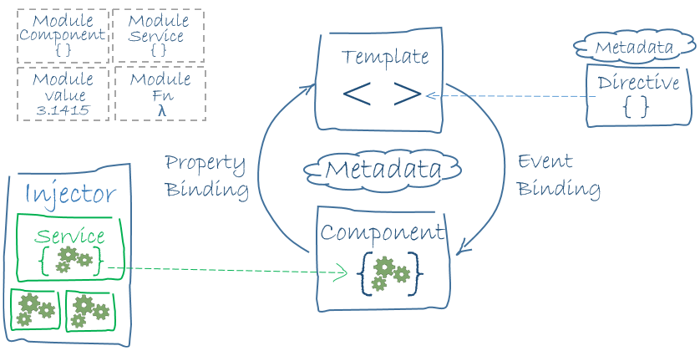
\includegraphics[height=0.5\linewidth]{angular.png}
\centering
\caption{Arhitectura platformei Angular.}
\label{fig:angular}
\end{figure} 